\subsection{Generalities}
DALES  is rooted in the LES of \citet{nieuwstadt1986}. \citet{cuijpers1993} first used DALES for moist convection, and provide a general description of an older version of DALES. Large parts of the code have been changed ever since and  contributions of many people over a number of years have resulted in the current version 3.2 of DALES. Currently, DALES is maintained by researchers from (alphabetically) Delft University, the Royal Netherlands Meteorological Institute (KNMI), and Wageningen University.

Notable changes in comparison with the version that has been described by \citet{cuijpers1993}, include: Different time integration and advection schemes, revised subfilter-scale, surface, and radiation schemes, addtion of a  cloud-microphysical scheme, capabilities for chemical reactive scalar transport and for Lagrangian particle dispersion, for flow over heterogeneous and for flow over sloped terrain. These revisions  in DALES result in faster simulations and higher stability, and in an easier and more extendable user interface. Due to the modular setup of the code, newly written code for specific applications of DALES can easily improve the code as a whole. This makes DALES suitable as a  community model; besides the actively developing core users, the model is currently used in several other institutes across the world.

DALES3.2 is released under the GPLv3 license. It is available at \url{www.ablresearch.org/dales} after registration. Documentation is also available there. Registration is necessary to keep track of the user base for dissemination of bug reports and fixes. Although the code is completely free to use, to modify and to redistribute, it is regarded courtesy to share bug fixes and extensions that can be of general interest, and to keep in contact with the core developers, also in case of publications.

DALES is written in Fortran 95. The only dependency of DALES are on makedepf90 for building (packeged with the code), and on the Message Passing Protocol (MPI). Some optional modules also require NetCDFv3. Code for Fourier transformations is provided as well, leaving DALES as portable as possible. To the best knowledge of the authors, DALES runs on all common combinations of platform architecture, compiler, and MPI implementation. Currently, an effort is being made to port DALES  to nVidia graphical processors, using CUDA \citep{griffith2009}.

The prognostic variables of DALES are the three velocity components $u_i$, the liquid water potential temperature $\theta_l$, the total water specific humidity $q_t$, the rain water specific humidity $q_r$, the rain droplet number concentration $N_r$, and up to 100 passive or reactive scalars. Because of the one-and-a-half order scheme that parameterizes sub-filter scale dynamics, the subfilter-scale turbulent kinetic energy (SFS-TKE, $e$) counts as an additional prognostic variable. To decrease simulation time, most prognostic variables can be switched of; only calculations of $u_i$, $e$, and $\theta_l$ are obligatory.

Given that ice is not currently implemented in the model, the total water specific humidity is defined as  the sum of the water vapor specific humidity $q_v$ and the cloud liquid water specific humidity $q_c$:
\begin{equation}
q_t = q_v + q_c
\end{equation}
 Note  that this definition excludes the rain water specific humidity $q_r$ from $q_t$. Any conversion between rain water on the one hand, and cloud water or water vapor on the other hand, will therefore enter the equations for $q_t$ and for $\theta_l$ as an addition source term. As a definition of $\theta_l$, we use the close approximation explained by \citet{emanuel1994}:
\begin{equation}
 \theta_l \approx \theta - \frac{L}{c_{pd}\Pi}q_c
\end{equation}
with $L=2.5\times10^6\mr{J\ kg^{-1}}$ the latent heat release of vaporization, $c_{pd}=1004\mr{J\ kg^{-1}\ K^{-1}}$ the heat capacity of dry air, and $\Pi$ the exner function:
\begin{equation}
\Pi = \left(\frac{p}{p_0}\right)^{\frac{R_d}{c_{pd}}}.
\end{equation}
In which $R_d=287.0 \mr{J\ kg^{-1}\ K^{-1}}$ is the gas constant for dry air.

 In the absence of precipitation and other explicit source terms, $\theta_l$ and $q_t$ are conserved variables. The virtual potential temperature $\theta_v$ is in good approximation defined with:
\begin{eqnarray}
\theta_v&\approx&\left(\theta_l+\frac{L}{c_{pd}\Pi}q_c\right)\left(1-\left(1-\frac{R_v}{R_d}\right)q_t-\frac{R_v}{R_d}q_c\right),
\end{eqnarray}
with $R_v=461.5 \mr{J\ kg^{-1}\ K^{-1}}$, the gas constants  for water vapor. The most important thermodynamical constants that are used throughout this paper are summarized in \tabnm \ref{tab:gov_thermoconst}
\begin{table}
\begin{center}
\begin{tabular}{|l|l|l|}
\hline
$R_v$ &Gas constant for water vapor&   $461.5 \mr{J\ kg^{-1}\ K^{-1}}$ \\
$R_d$ &Gas constant for dry air&   $287.0 \mr{J\ kg^{-1}\ K^{-1}}$ \\
$L$ &Latent heat release for vaporization&   $2.5\times10^6\mr{J\ kg^{-1}}$ \\
$c_{pd}$ &Heat capacity for dry air&   $1004\mr{J\ kg^{-1}\ K^{-1}}$ \\
\hline
\end{tabular}
\end{center}
\caption{\label{tab:gov_thermoconst} The main thermodynamical constants used throughout this paper.}
\end{table}

DALES assumes the Boussinesq approximation, and is run on an Arakawa C-grid (see \fignm \ref{fig:cgrid}). The pressure, the SFS-TKE, and the scalars are defined at cell center, the 3 velocity components are defined at the West side, the South side, and the bottom side of the grid cell, respectively.

In the remainder of this article, quantities that are averaged over the LES-filter are denoted with a tilde $\fav{\cdot}$, time averages with a overbar $\tav{\hspace{0.5ex}\cdot\hspace{0.5ex}}$, and averages over the two horizontal directions of the domain with angular brackets $\xav{\cdot}$ (slab average). The prognostic scalars can often be treated simultaneously as the generic scalar field $\varphi \in\{ \theta_l, q_t, q_r,N_r,s_n\}$.  Primes denote the subfilter-scale fluctuations with respect to the filtered mean. To remain consistent with notational conventions as used in literature and also in the source code of DALES, some symbols can have different meaning between different subsections. In such cases, the immediate context should always make it clear what each symbol stand for in a particular section. Vertical velocities and fluxes are in general directed upward; only the radiative and sedimentation fluxes point downward, following conventions.

\subsection{The governing equations}
Within the Boussinesq approximation the equations of motion, after application of the LES filter, are given by
\begin{eqnarray}
\label{eq:comp_continuity}
\derr{\fav{u_i}}{x_i} &=& 0,\\
\label{eq:comp_RANS}
\derr{\fav{u_i}}{t} &=& - \derr{\fav{u_i}\fav{u_j}}{x_j}-\derr{\pi}{x_i} + \frac{g}{\theta_0}(\fav{\theta_v}-\theta_0)\delta_{i3} + \force{i}{}- \derr{\tau_{ij}}{x_j},\\
\label{eq:comp_varphi}
\derr{\fav{\varphi}}{t} &=& - \derr{\fav{u_j}\fav{\varphi}}{x_j}- \derr{R_{u_j,\varphi}}{x_j}+\mathcal{S}_{\varphi},
\end{eqnarray}
where the tildes denotes the filtered mean variables. Viscous transport terms have been neglected. The z-direction ($x_3$) is taken to be vertical. $\theta_0$ is the reference state potential temperature and  $\force{i}{}$ represents other forcings, including large scale forcings and the Coriolis forcing
\begin{equation}
 \force{i}{cor} = - 2\epsilon_{ijk}\Omega_j\fav{u_k},
\end{equation}
where $\vec{\Omega}$ is the earth's angular velocity. Source terms for scalar $\varphi$ are denoted by $\source{\varphi}{}$, and may include of microphysical ($\source{}{mcr}$), radiative ($\source{}{rad}$), chemical ($\source{}{chem}$), large-scale ($\source{}{ls}$), and relaxation ($\source{}{rel}$) terms.  The subfilter-scale (SFS), or residual, scalar fluxes are denoted by $R_{u_j,\varphi}\equiv\fav{u_j \varphi}-\fav{u_j}\fav{\varphi}$, i.e., the contribution to the resolved motion from all scales below the LES filter width. The anisotropic SFS-stress tensor is defined by
\begin{equation}
 \tau_{ij}\equiv \fav{u_iu_j}-\fav{u_i}\fav{u_j}-\frac{2}{3}\delta_{ij}\sgse,
\end{equation}
where $\sgse=\frac{1}{2}(\fav{u_iu_i}-\fav{u_i}\fav{u_i})$ is the subfilter-scale turbulent kinetic energy (SFS-TKE). Formally, the trace of the SFS-stress has been included in the modified pressure
\begin{equation}
\pi=\frac{1}{\rho}(\fav{p}-p_0)+\frac{2}{3}e.
\end{equation}
To enforce continuity (\eqnm  \ref{eq:comp_continuity}), a Poisson equation for $\pi$ is solved
\begin{eqnarray}
\derr{^2\pi}{x_i^2} &=& \derr{}{x_i}\left(- \derr{\fav{u_i}\fav{u_j}}{x_j}+ \frac{g}{\theta_0}({\theta_v}-\theta_0)\delta_{i3} \iftwocol{\right.\nonumber\\&&\left.}{}-2\epsilon_{ijk}\Omega_j\fav{u_k}+ \force{i}{}- \derr{\tau_{ij}}{x_j}\right).
\end{eqnarray}
Since computations are performed in a double periodic domain, the Poisson equation is solved by applying a Fast Fourier Transform in the homogenous directions followed by solving a tridiagonal system in the $z$-direction. A schematic overview of how the different processes affect the different variables is given in \fignm \ref{fig:flowchart}.
\begin{figure}
 \begin{center}
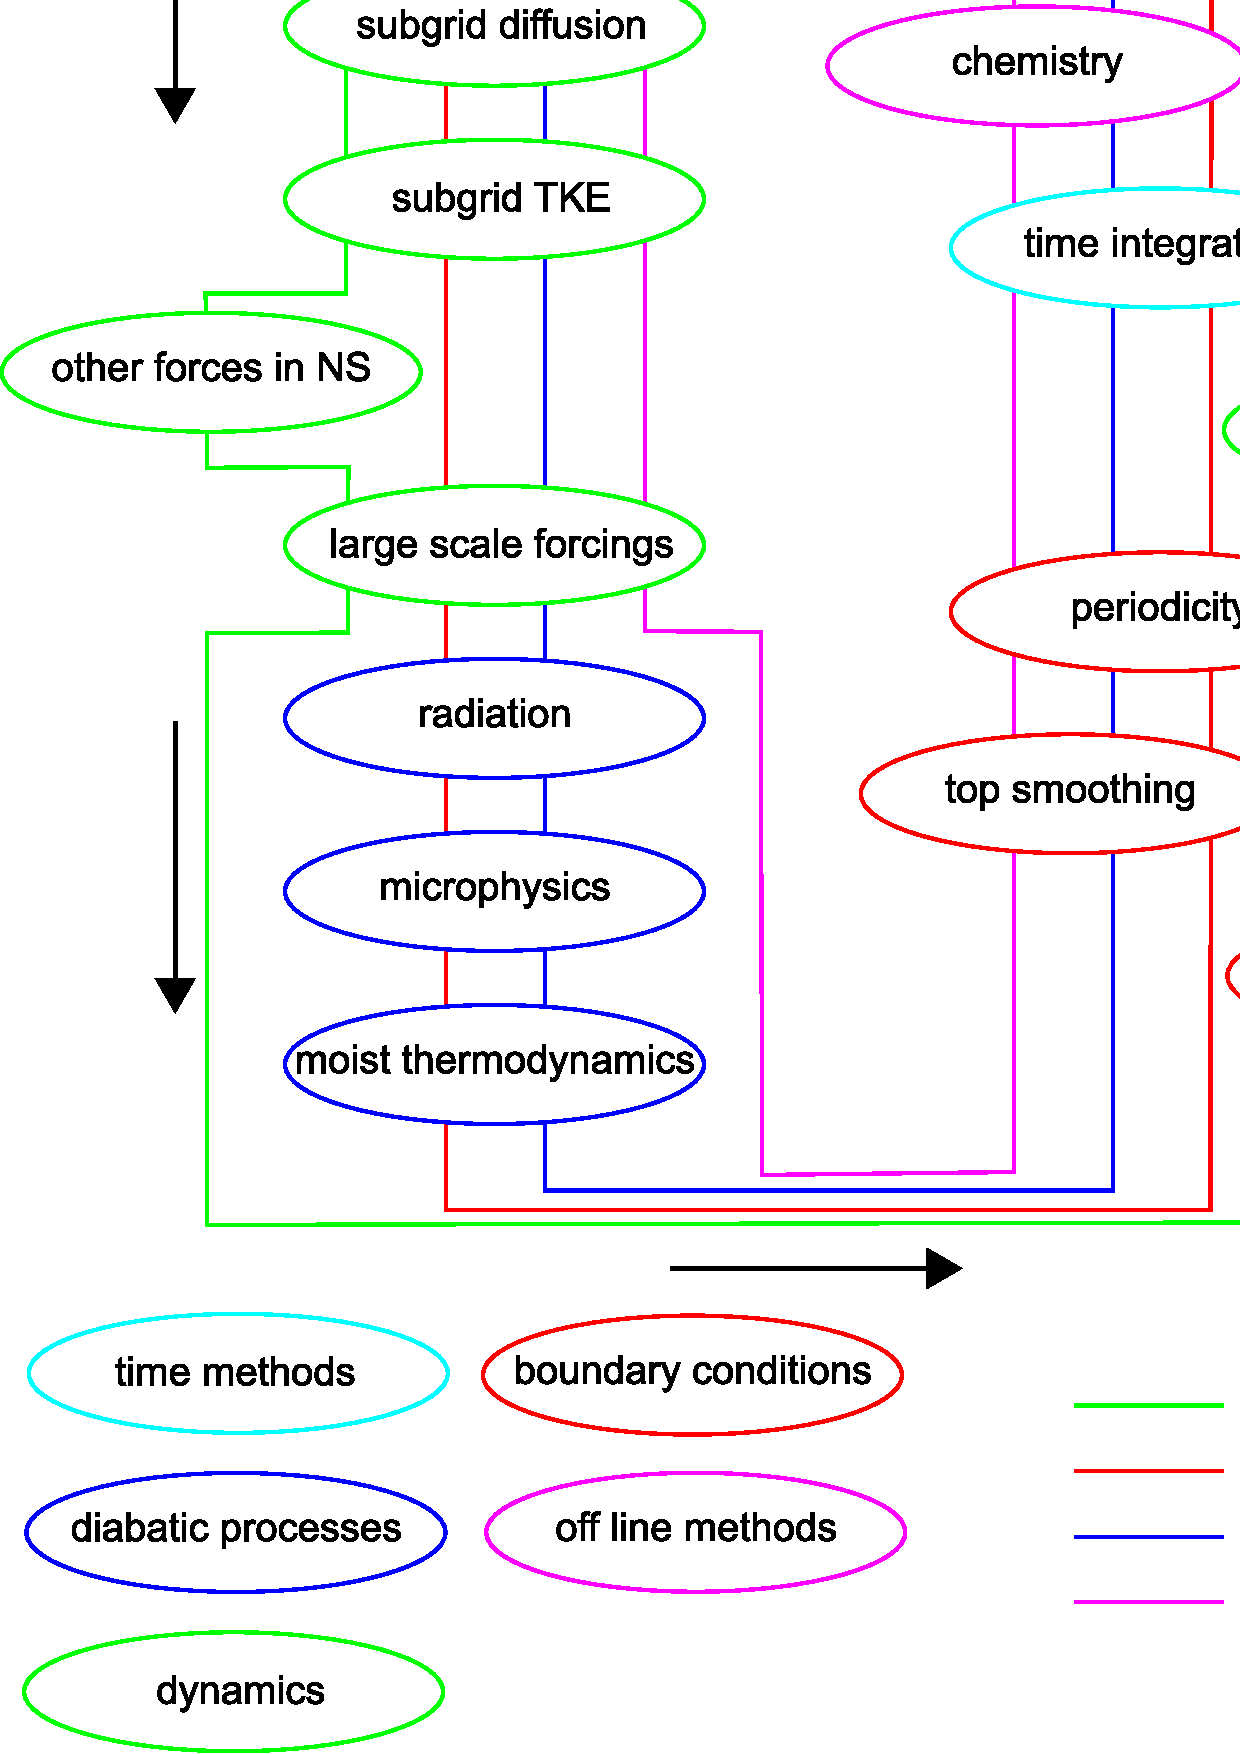
\includegraphics[width=0.45\textwidth]{fig_flowchart}
\caption{Flowchart of DALES.}
\label{fig:flowchart}
\end{center}
\end{figure}

